\documentclass[12pt]{exam}
\usepackage{epsfig}
\usepackage[usenames,dvipsnames,svgnames,table]{xcolor}
\usepackage{listings}
\usepackage{color}
\usepackage{float}
%\usepackage{enumitem}
\usepackage{bookmark}
\usepackage{paralist}

% Must be last
\usepackage{hyperref}

\hypersetup{
    colorlinks=true,
    linkcolor=blue,
    filecolor=magenta,
    urlcolor=blue,
}

\newcommand{\note}[1]{\marginpar{\LARGE $\spadesuit$}
      $\spadesuit$ {\bf #1} $\spadesuit$}
      
\lstdefinestyle{error}{
  emptylines=1,
  breaklines=true,
  basicstyle=\ttfamily\color{red}
}

\lstdefinestyle{command}{
  emptylines=1,
  breaklines=true,
  basicstyle=\ttfamily\color{black}
}


\pagestyle{headandfoot}
\firstpageheader{}{}{}
\runningheader{CPSC 314}{Assignment 3}{Due March 11th, 2022}
\setlength{\parindent}{0pt}
\begin{document}

\title{CPSC 314\\
  Assignment 3: Shaders}
\date{Due 11:59PM, March 11th, 2022}

\maketitle 

\section{Introduction}

In this Assignment, you will utilize your knowledge of lighting and shading to modify the appearance of 3D models.
Here we will study how to use basic textures and implement various shading algorithms: Blinn-Phong, Toon, as well as some other fun shaders. This is a rather interesting assignment, so we hope you will have fun with this one.

\subsection{Getting the Code}
Assignment code is hosted on the UBC Students GitHub. To retrieve it
onto your local machine navigate to the folder on your machine where you intend to keep your
`assignment code, and run the following command from the terminal or command line:

\medskip
{\tt git clone https://github.students.cs.ubc.ca/cpsc314-2021w-t2/a3-release.git}



\subsection{Template}
\begin{itemize}
\item The file {\tt A3.html} is the launcher of the assignment. Open
  it in your preferred browser to run the assigment, to get started.
\item The file {\tt A3.js} contains the JavaScript code used to set up the scene and the rendering environment. You will need to make minor in it to answer the questions.
\item The folder {\tt glsl} contains the vertex and fragment shaders for the armadillo and other geometry. This is where you will do the rest of your coding.
\item The folder {\tt js} contains the required JavaScript libraries. You do not need to change anything here.
\item The folder {\tt obj} contains the geometric models loaded in the scene.
\item The folder {\tt images} contains the texture images used.
\end{itemize}

\subsection{Execution}
As mentioned above, the assignment can be run by opening the file {\tt
  A3.html} in any modern browser. However, most browsers will prevent
pages from accessing local files on your computer. If you simply open
{\tt A3.html}, you may get a black screen and an error message on the
console similar to this:
\begin{lstlisting}[style = error]
    XMLHttpRequest cannot load... Cross origin requests are only supported for protocol schemes: http, data, https.
\end{lstlisting}

Please see this web page for options on how to run things locally:
\begin{quotation}
    {\footnotesize \url{https://threejs.org/docs/\#manual/en/introduction/How-to-run-things-locally}}
\end{quotation}

% We highly recommend that you run a local server, instead of changing browser security settings.

% \begin{enumerate}
%     \item Follow the link \url{https://nodejs.org/en/} to download and install Node.js, which
%         comes packaged with npm.
%     \item Open the link \url{https://www.npmjs.com/package/http-server} and follow the
%         instructions to download and install a local command-line http server.
%     \item Go to the command-line or terminal and run {\tt http-server [path]}
%         where [path] is the path to the assignment folder.
%     \item Open your preferred browser and copy and paste the URL of the
%         local server specified by the http-server on your command-line.
% \end{enumerate}

% \newpage

\section{Work to be done (100 pts)}

First, ensure that you can run the template code in your browser. See instructions in Assignment 1. The initial scene should look as in Figure 1. Study the template to get a sense of what and how values are passed to each shader file. There are four scenes, each corresponding
to a different shader, you may toggle between them using the number keys 1, 2, 3 on
your keyboard: 1: Blinn-Phong, 2: Toon, 3: Rolling Grid.

\vspace{0.5cm}

The default scene is set to 1. See
\begin{quotation}
\verb|let mode = shaders.PHONG.key;|
\end{quotation}
in A3.js. You may find  
it convenient during your development to change this default value to the scene containing
the shader that you are currently working on (e.g., for question 1b, you could use
\verb|let mode = shaders.TOON.key;|).

\begin{figure}[H]
    \centering
    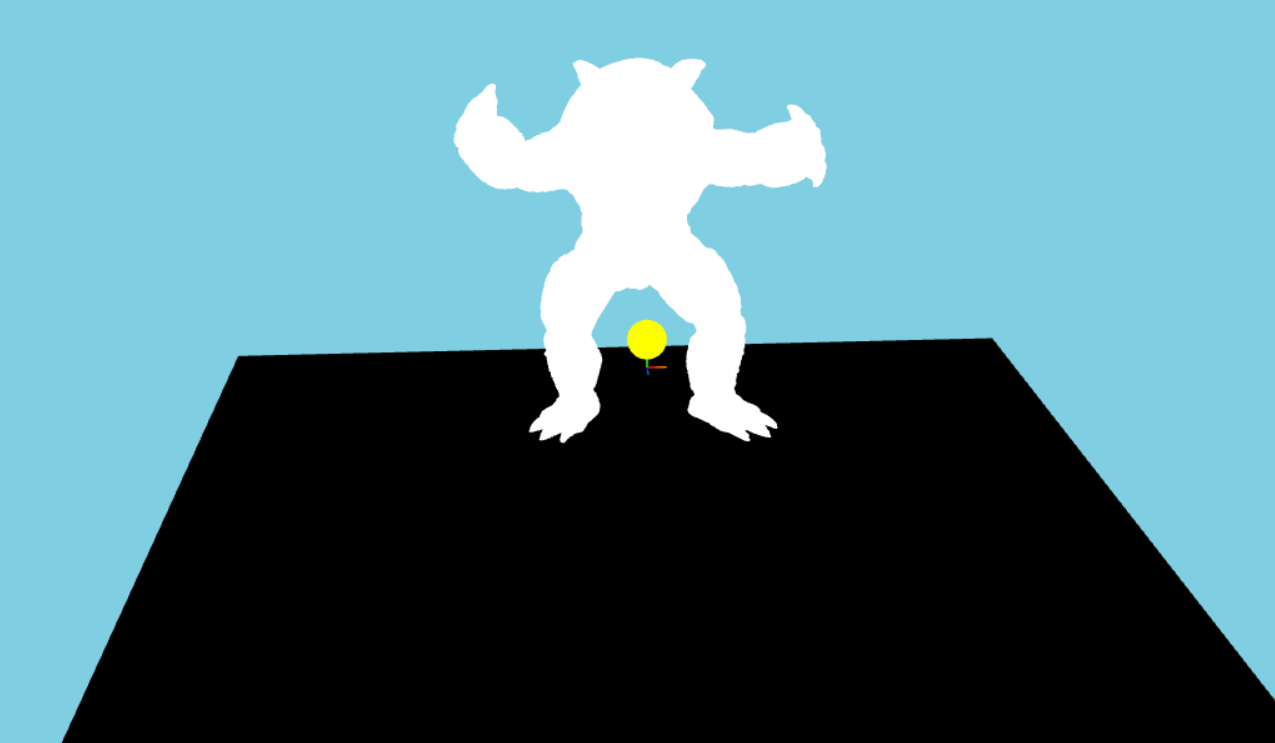
\includegraphics[width=0.3\textwidth]{./init.png}
    \caption{Initial configuration}
\end{figure}

\clearpage

{\bf Part 1: Required Features}


\begin{description}
  
\item [(a)] {\bf 15 pts} Basic Texturing
\label{ref:simpleorb}

For the first part of the assignment, you will implement a basic texturing.  Your goal is to use the provided floorColorTexture
to give the floor a rocky appearance. Use the provided floor vertex and fragment shaders, with the appropriate uniforms, to sample
and apply the texture. 

    \begin{figure}[H]
    \centering
    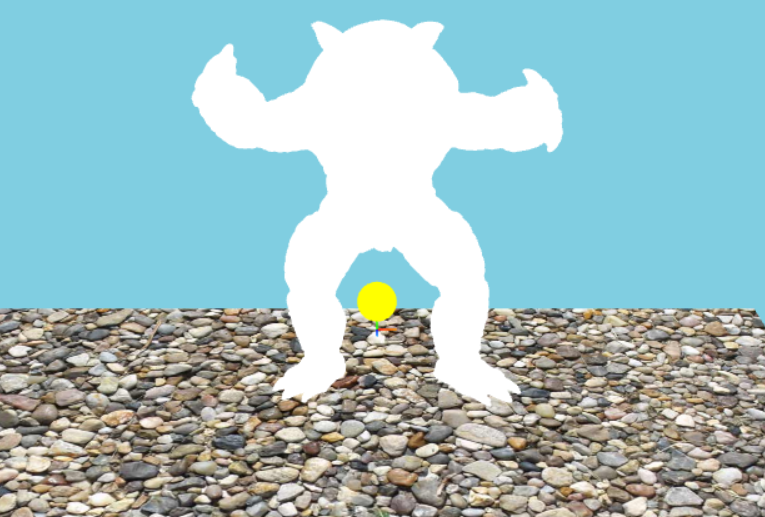
\includegraphics[width=0.8\textwidth]{./q1.png}
    \caption{Question 1(a). Textured floor}
    \end{figure}

\item[(b)] {\bf 25 pts} Blinn-Phong Reflection
\label{ref:simpleorb}

  First of all, note that the Phong reflection model is a different type of thing
than the Phong shading model; they just happen to be named after the same
person. The latter improves on the Gouraud shading by computing the lighting
per fragment, rather than per vertex. This is done by using the interpolated values
of the fragment’s position and normal. We’ll be using Phong shading throughout
this assignment except for part 1 (d). The
following image, taken from the Wikipedia article on this model, shows how the
different components look individually and summed together:
    \begin{figure}[H]
    \centering
    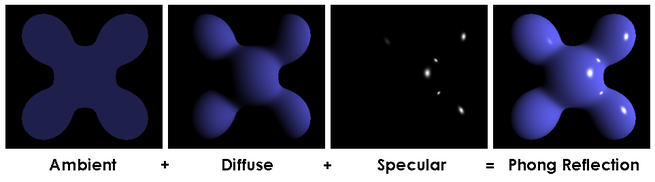
\includegraphics[width=0.8\textwidth]{./pic2.png}
    \caption{Phong reflection model.}
    \end{figure}
In this scene, you’ll implement the Blinn-Phong reflection model, which is a 
slight modification of the specular component of Phong's original reflection model 
to make it more compatible with physically-based rendering (we will cover that later in the course).
It is also simpler, and described in detail (with code) in the textbook, Section 1.3; it uses the ``halfway vector,'' instead of the ``bounce'' vector. 

  \textit{Hint 1: }This part can be done entirely in {\tt phong.fs.glsl} and {\tt phong.vs.glsl}. 
    
Your task here is to complete the code in phong.vs.glsl and phong.fs.glsl
to shade the Armadillo in Scene 1 using the Blinn-Phong reflection algorithm. The
main calculations should all go in the fragment shader, but you will still need a
vertex shader to pass the appropriate information to your fragment shader. Your
resulting armadillo should look something like Figure \ref{fig:phong}.

    \begin{figure}[H]
    \centering
    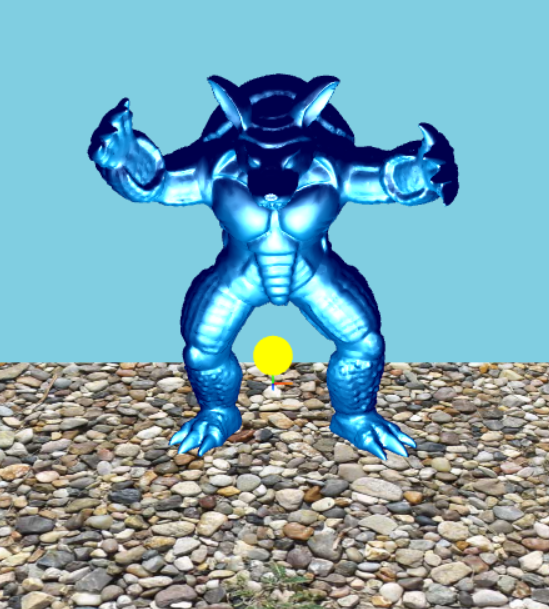
\includegraphics[width=0.35\textwidth]{./q2.png}
    \caption{Question 1(b). Blinn-Phong'd armadillo \label{fig:phong}}
    \end{figure}
    
\clearpage
    
\item [(c)] {\bf 25 pts} Toon
\label{ref:simpleorb}

Send the armadillo to the realm of action and superheros! Unlike the smooth, realistic shading in the previous questions, Toon shading gives a non-photorealistic
result. It emulates the way cartoons use very few colors for shading, and the color
changes abruptly, while still providing a sense of 3D for the model. This can be
implemented by quantizing the light intensity across the surface of the object.
Instead of making the intensity vary smoothly, you quantize this variation into a
number of steps for each “layer” of toon shading.
Use two blue colour tones for the armadillo (lower light intensity will be a darker shade), as seen in Figure 4.

\vspace{0.2cm}

This is most easily done by interpolating between two predefined colours. Lastly,
draw a dark blue silhouette on the armadillo. You can use the cosine of the
normal and the viewing direction to compute whether the fragment should be an
outline: fragments that are “edgy” enough should be outlines, and recall how you
can obtain the cosine for two vectors.

\vspace{0.2cm}

If you need some inspiration, the following movies and video games were rendered with toon shading (also called cell shading) techniques:

{\tt http://en.wikipedia.org/wiki/List\_of\_cel-shaded\_video\_games}

\textit{Hint 1: } Use the surface normal and the viewing direction of a fragment to determine whether it is on the silhouette of the armadillo.

\textit{Hint 2: } Since the silhouette is determined using the surface normal and the
viewing direction, and does not depend the light direction, moving the light source
will not affect its location.

    \begin{figure}[H]
    \centering
    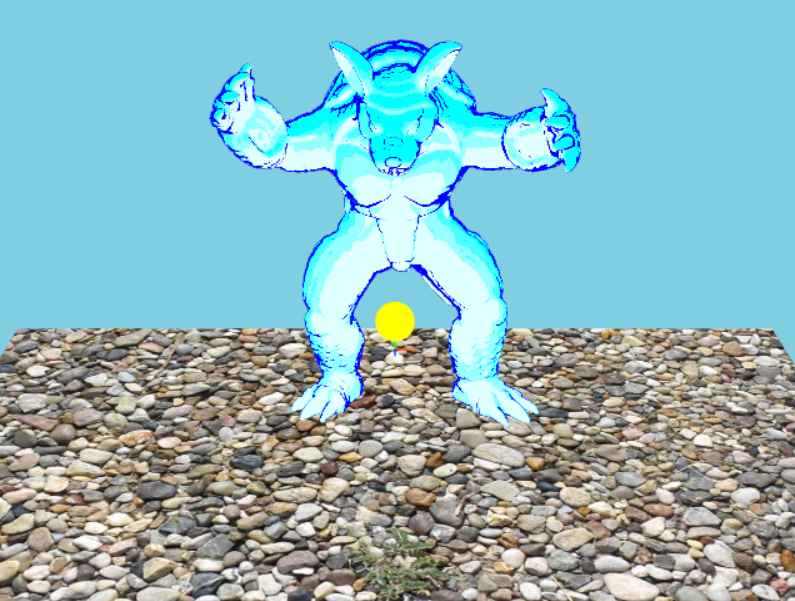
\includegraphics[width=0.35\textwidth]{./q3i.png}
    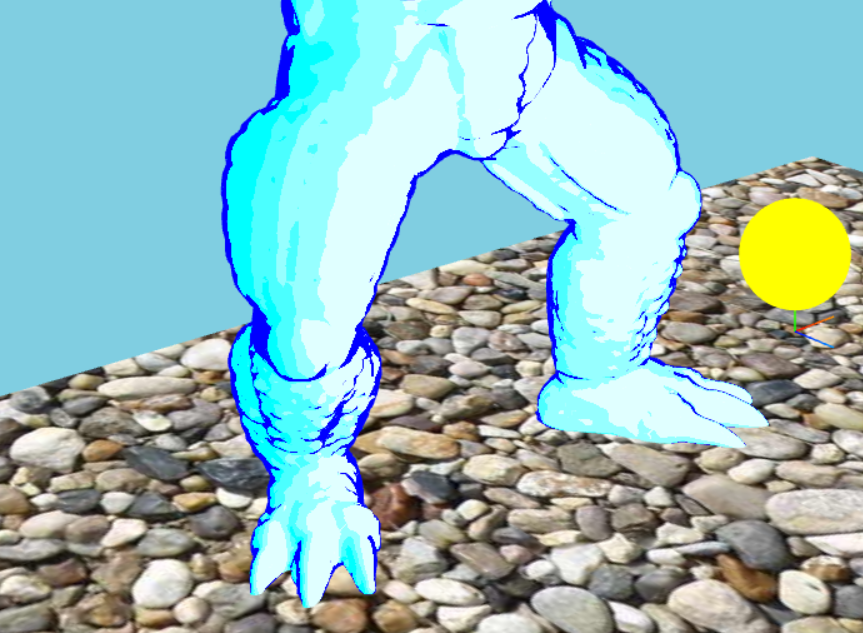
\includegraphics[width=0.35\textwidth]{./q3ii.png}
    \caption{Question 1(c). Toon armadillo}
    \end{figure}

\clearpage

\item[(d)] {\bf 35 pts} Scene 3: Grid pattern

  The possibilities are endless! Here, we will (i) make the armadillo
  out of squares by checking whether a fragment is close enough to planes
  on a regular grid in the 3D space around the armadillo; (ii) make
  the grid squares smoothly ``roll'' down the body over time, as in
  Figure \ref{fig:gridpattern}, and (iii) interpolate the color of the fragments
  by the light intensity. To do so, you will need to write a function in the fragment
  shader that shades the fragment depending on a time ``ticks'' and
  the local vertex position, discarding fragments that you don't want
  to render. Notice the empty space between the grid squares. Complete the
  code in squares.vs.glsl and squares.fs.glsl.

    \textit{Hint 1: }: The {\tt discard} statement in GLSL throws away the current fragment, so
    it is not rendered.
    
    \textit{Hint 3: }: The armadillo's model coordinates may be
    smaller than you think. If your armadillo disappears completely
    (not because of some syntax error) try using smaller numbers when
    computing regions to discard.
    
    \begin{figure}[H]
    \centering
    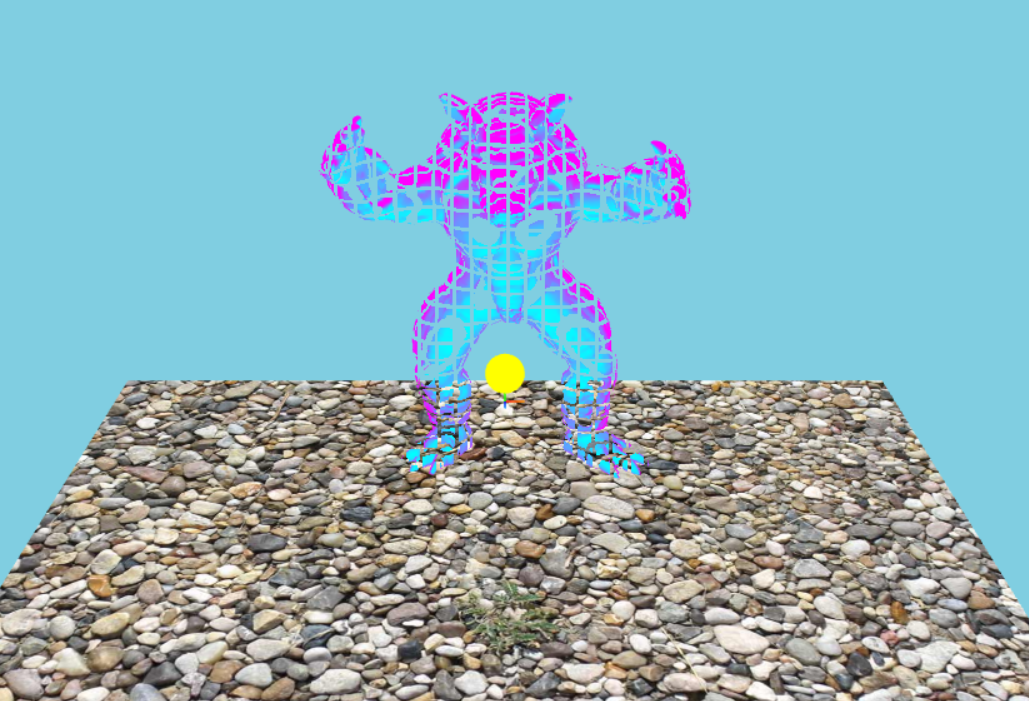
\includegraphics[width=0.35\textwidth]{./q4.png}
    \caption{Question 1(d). Grid-pattern armadillo \label{fig:gridpattern}}
    \end{figure}

\newpage

\end{description}

\clearpage

{\bf Part 2: Creative License (Optional)}

You have many opportunities to unleash your creativity in
computer graphics!  In this \textbf{optional} section, and you are
invited to extend the assignment in fun and creative ways.
We'll highlight some of the best work in class. A small number of
exceptional contributions may be awarded bonus points.
Some possible suggestions might be:
\begin{itemize}
\item Create a new interesting shader for the armadillo or
  chest. E.g., Make the armadillo's skin out of an anisotropic
  material, like brushed metal. e.g., see using Heidrich-Seidel
  Anisotropic distribution model
  \\
  {\footnotesize
\verb|https://en.wikipedia.org/wiki/Specular_highlight#Heidrich%E2%80%93Seidel_anisotropic_distribution|}

\item Add a new object that uses texture mapping.

\item Generate new animated effects using the {\tt discard} function in GLSL.


\end{itemize}


\section{Submission Instructions}
\subsection{Directory Structure}
Under the root directory of your assignment, create two subdirectories
named ``part1'' and ``part2'', and put all the source files and everything
else required to run each part in the respective folder. Do not create more
sub-directories than the ones already provided. 

You must also write a clear README.txt file that includes your name,
student number, and CWL username, instructions on how to use the
program (keyboard actions, etc.) and any information you would like to
pass on to the marker. Place README.txt under the root directory of your
assigment.

\subsection{Submission Methods}
Please compress everything under the root directory of your assignment into
{\tt a3.zip} and submit it on Canvas. You can make multiple submissions,
but we will grade only the last one.

\section{Grading}
\subsection{Point Allocation}
Each assignment has 100 points for Part 1. Part 2 is optional and you can get bonus points (0-10 points) at the
instruction team's discretion.
Percentage wise, we use Part 1's total points as the denominator: e.g. if you
get 95 out of 100 points from Part 1, but no points from Part 2, then your percentage
grade would be 95/100. If you get full points from both Parts, then your percentage
grade would be 110/100.

\subsection{Face-to-face (F2F) Grading}
For each assignment, you are required to meet face-to-face with a TA on Zoom or in person
to demonstrate that you understand why your program works. Details regarding how to
sign up a grading session with a TA will be announced on Canvas and on Piazza.

\subsection{Penalties}
Aside from penalties from incorrect solution or plagiarism, we may apply the following
penalties to each assignment:

\textbf{Late penalty.} You are entitled up to three grace (calendar) days in total
throughout the term. No penalties would be applied for using them. However once
you have used up the grace days, a deduction of 10 points would be applied to each
extra late day. Note that
\begin{enumerate}
  \item The three grace days are given for all assignments, \textbf{not per assignment}, so please use them wisely;
  \item We consider the time of only your last submission;
  \item We do not consider Part 1 and Part 2 submissions separately. Say if you submitted Part 1 on time but updated your submission for Part 2 one day after the deadline, we would count one late day.
\end{enumerate}

\textbf{No-show penalty.} You are required to sign up a grading slot at least one day
before F2F grading starts, and show up at your slot on time. So a 10-point deduction would
be applied to each of the following circumstances:
\begin{enumerate}
  \item Not signing up a grading slot before the sign-up period closes;
  \item Not showing up at your grading slot.
\end{enumerate}
Note that we would not apply the no-show penalty if you are unable to sign up/show up on
time due to an emergency, or if you cannot sign up because none of the slots work for you.
In those cases, please contact the course staff on Piazza before a sign-up closes. If you have
not signed up on time or if you have missed your slot, please follow the steps outlined in
this Piazza post: {\footnotesize \url{https://piazza.com/class/ky4qwpnvrqa5pq?cid=190}}

\end{document}
%%% Local Variables:
%%% mode: latex
%%% TeX-master: t
%%% End:
